% Argue why anonymity is important
Location data is extremely sensitive but also useful for many applications.
In his survey of computational location privacy~\cite{krumm2009survey}, Krumm lists four main methods of protecting location privacy while still using location data:
% Duckham, M. and L. Kulik, Location privacy and location-aware
% computing, in Dynamic & Mobile GIS: Investigating Change in
% Space and Time, J. Drummond, et
\begin{enumerate}
  \item Anonymity
  \item Obfuscation
  \item Regulatory strategies
  \item Privacy policies
\end{enumerate}
Anonymizing a user ID associated with location data may sound good in theory, but due to the fact that a typical users movements are very unique, many attacks can re-identify these users in practice.
This raises the question: when can anonymized location data be used or released without fear of de-anonymization?
In this section, we explore the difficulties in anonymizing location data.
% Cite: Eckersley stuff, ideas for protecting location privacy from candidacy


\subsection{Related Work}

\begin{figure}[t]
  \centering
  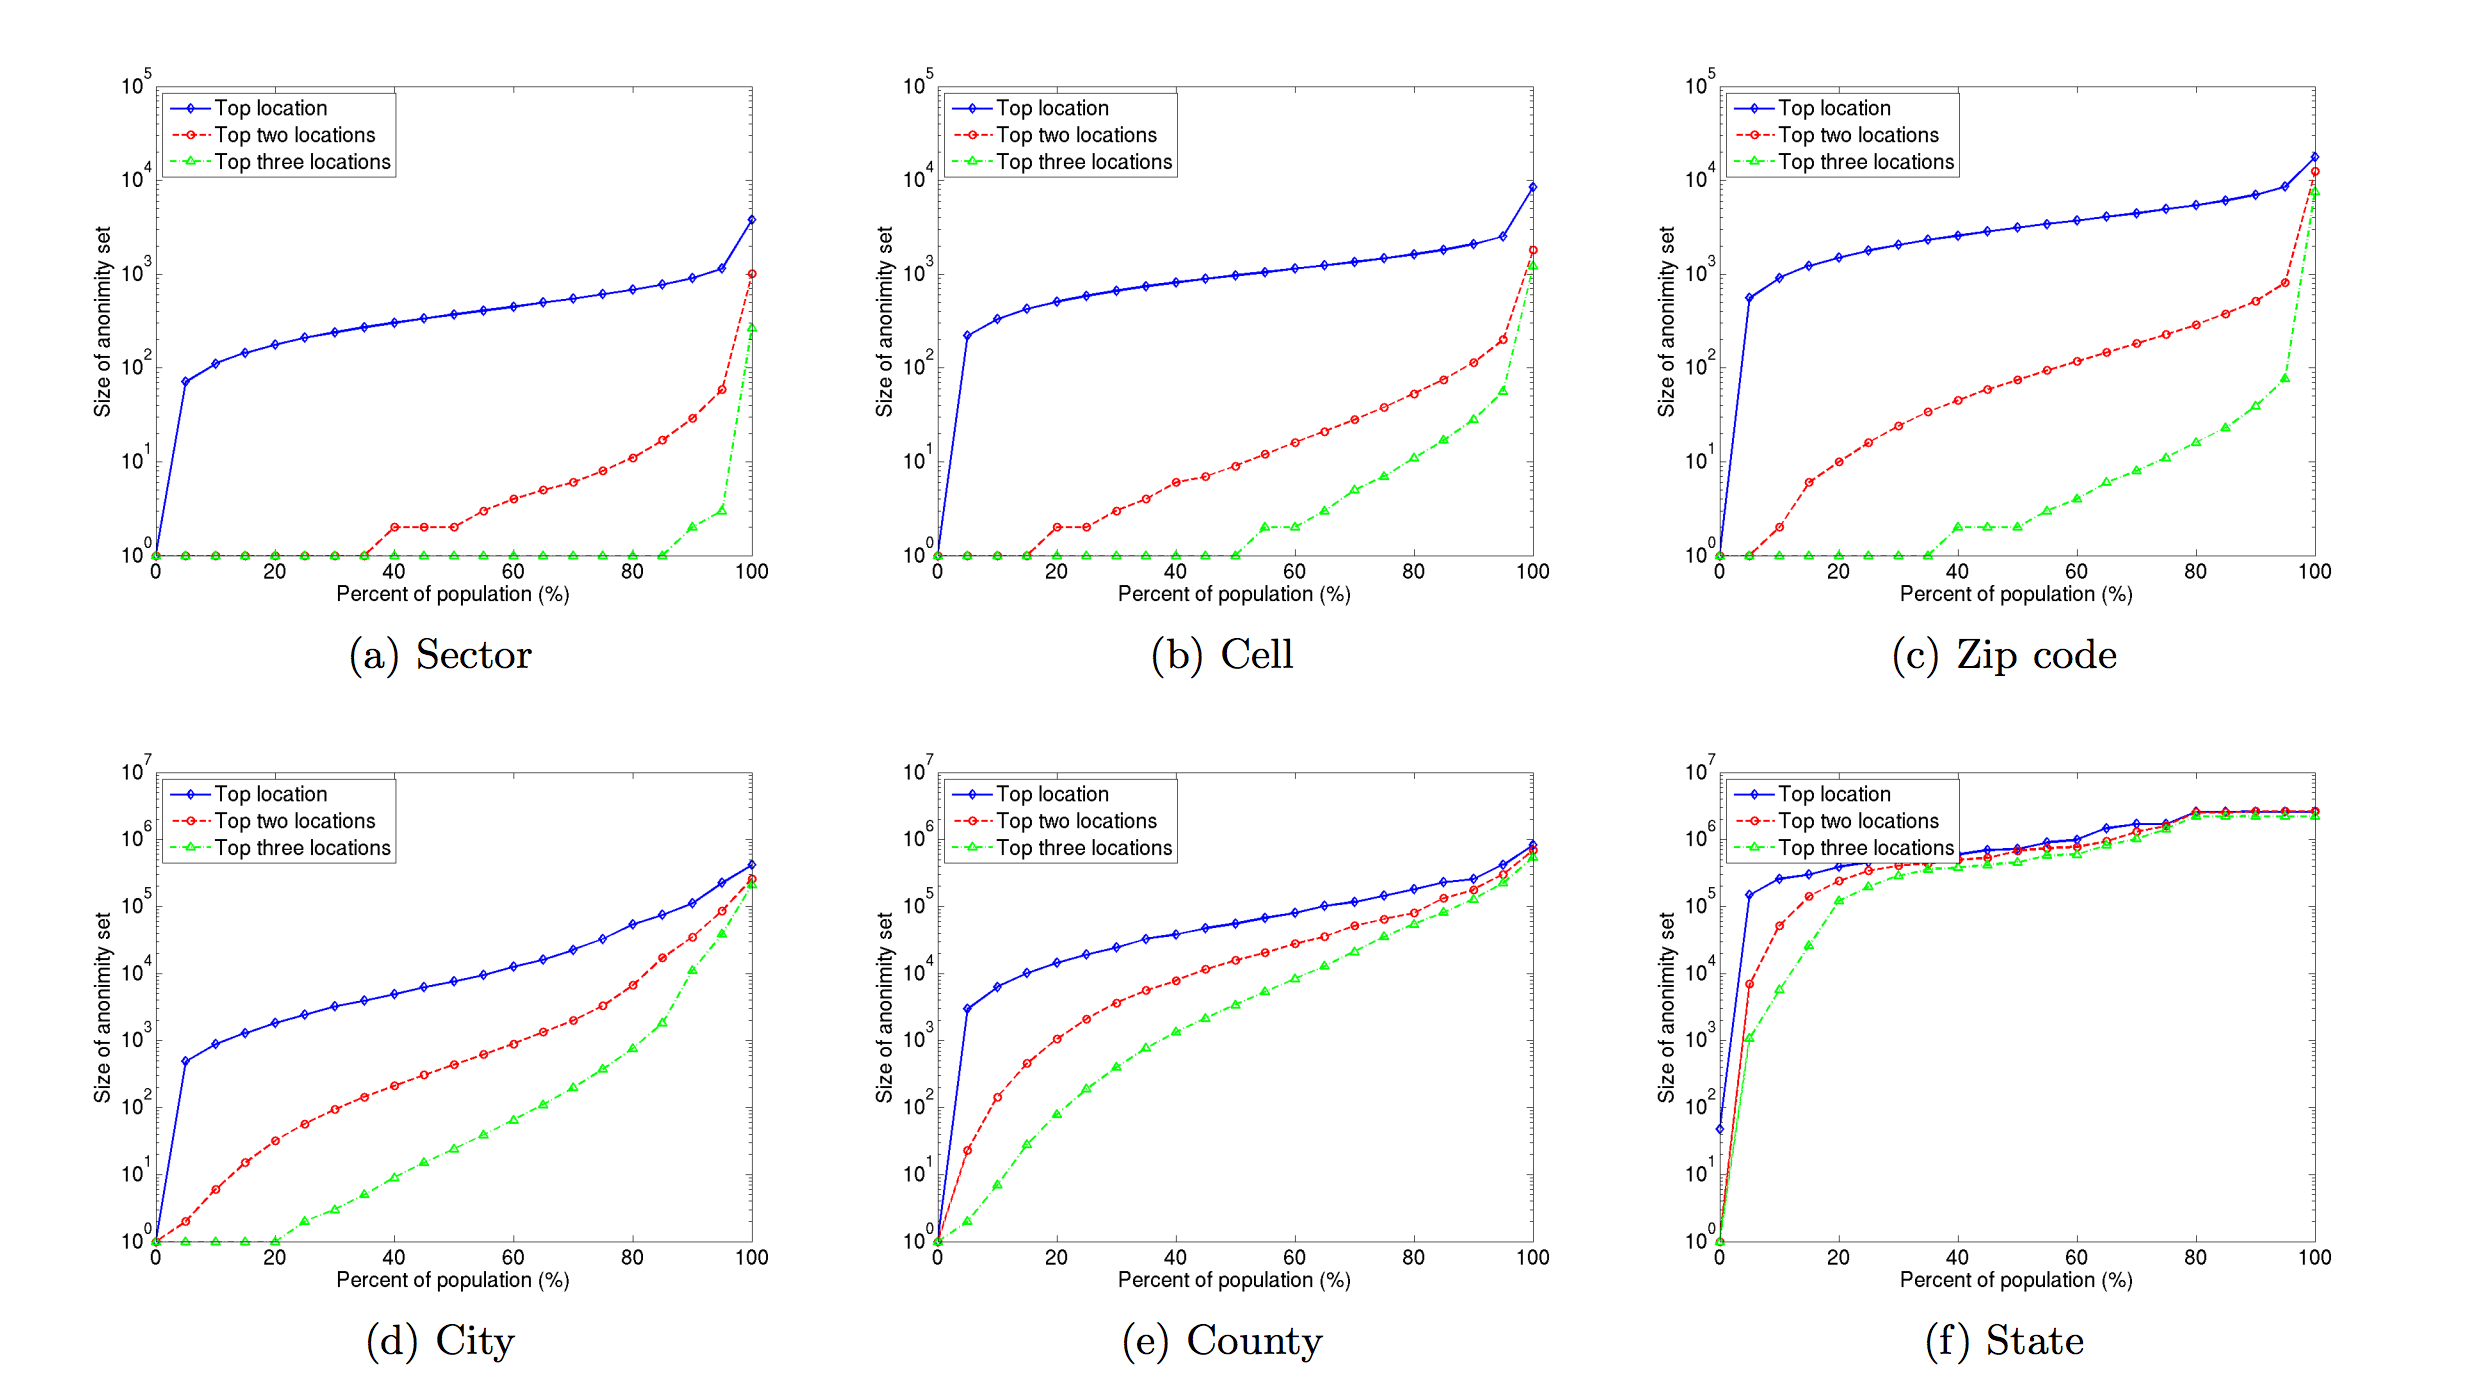
\includegraphics[width=\linewidth]{fig/zang_bolot.png}
  \caption{Figure from~\cite{Zang:2011hk} depicting the size of anonymity sets for top $n$ most visited location of users.
           Locations are varied in granularity, from cell sectors to US states.}
  \label{fig:zang_bolot}
\end{figure}

Location data for individuals is highly unique and thus difficult to anonymize.
The first large-scale study of the $k$-anonymity of location data was appropriately titled ``Anonymization of Location Data Does Not Work"~\cite{Zang:2011hk}.
The paper used data from cell phone call detail records (or CDR, see~\chap{sec:background}) for 25 million United States users over a 3 month period.
The authors represents each user as simply their top $n$ most visited locations, varying $n$ from 1 to 3.
Additionally, the authors varied the granularity of the locations, with the smallest as cell sector and the largest as state.
Remarkably, using 3 locations at a cell level made half of all users completely unique, and 3 locations a sector level made 85\% of all users unique.
A figure detailing this result and results for other granularities and values of $n$ is depicted in~\fig{fig:zang_bolot}.
The authors went on to analyze the impact of geography (comparing different states and cities), mobility (distances between top locations), and social networks on anonymity.

A different study used randomly selected points from a user's dataset and included time of location visit~\cite{de2013unique}, as opposed to a users top $n$ locations (mostly omitting precise time) of Zang and Bolot.
Using a call detail record dataset of 1.5 million users from a small European country, this work showed that 95\% of users are uniquely identified by 4 spatio-temporal points.
% TODO: add figure?
A follow up study~\cite{de2015unique} showed that in a data set of credit card transactions, user profiles of spatiotemporal points had a similar level of uniqueness, and even more when transaction amounts were included as well.


\subsection{Linking Users Across Domains with Location Data}
% Background...
Although prior work showed location to be highly \emph{unique} and thus possibly \emph{vulnerable} to de-anonymization, no data was actually de-anonymized in practice.
Indeed, just because a data source is highly unique does not mean it can be de-anonymized.
To put it more concretely, imagine that each individual had a die with 1000 sides, and each side represented a location.
For example, much of cryptography relies on creating unique but unpredictable sequences of numbers.
If, quite hypothetically, humans decided where to go next by rolling this die, their movements would look very unique.
However, since the movements are random and unpredictable, my movements from different time periods will be indistinguishable from those of a different individual.

TODO: put some math here?

Another possibile break in the argument that uniqueness implies vulnerability is the important factor of sampling.
The datasets dealt with here (phone records, social media posts) are all \emph{actively} collected: each data point exists if and only if the user has taken an action.
Intuitively, the location data from different sampling data sources should look very different.
An individual may be more likely to make phone calls in quiet places, like the home or office, and take geotagged location photos in popular tourist destinations or restaurants.

TODO: put some math here?

The vector of attack implied in the above-mentioned works are having access to an original, anonymized dataset, and then de-anonymizing it with a subset of auxiliary information with columns identical to the original set.
In ``Linking Users Across Domains with Location Data", published at WWW in 2016~\cite{riederer2016linking}, we tackled the problem of linking users across two entirely different datasets using only their location data.

% Describe problem setting
\begin{figure*}[t]
  \begin{center}
    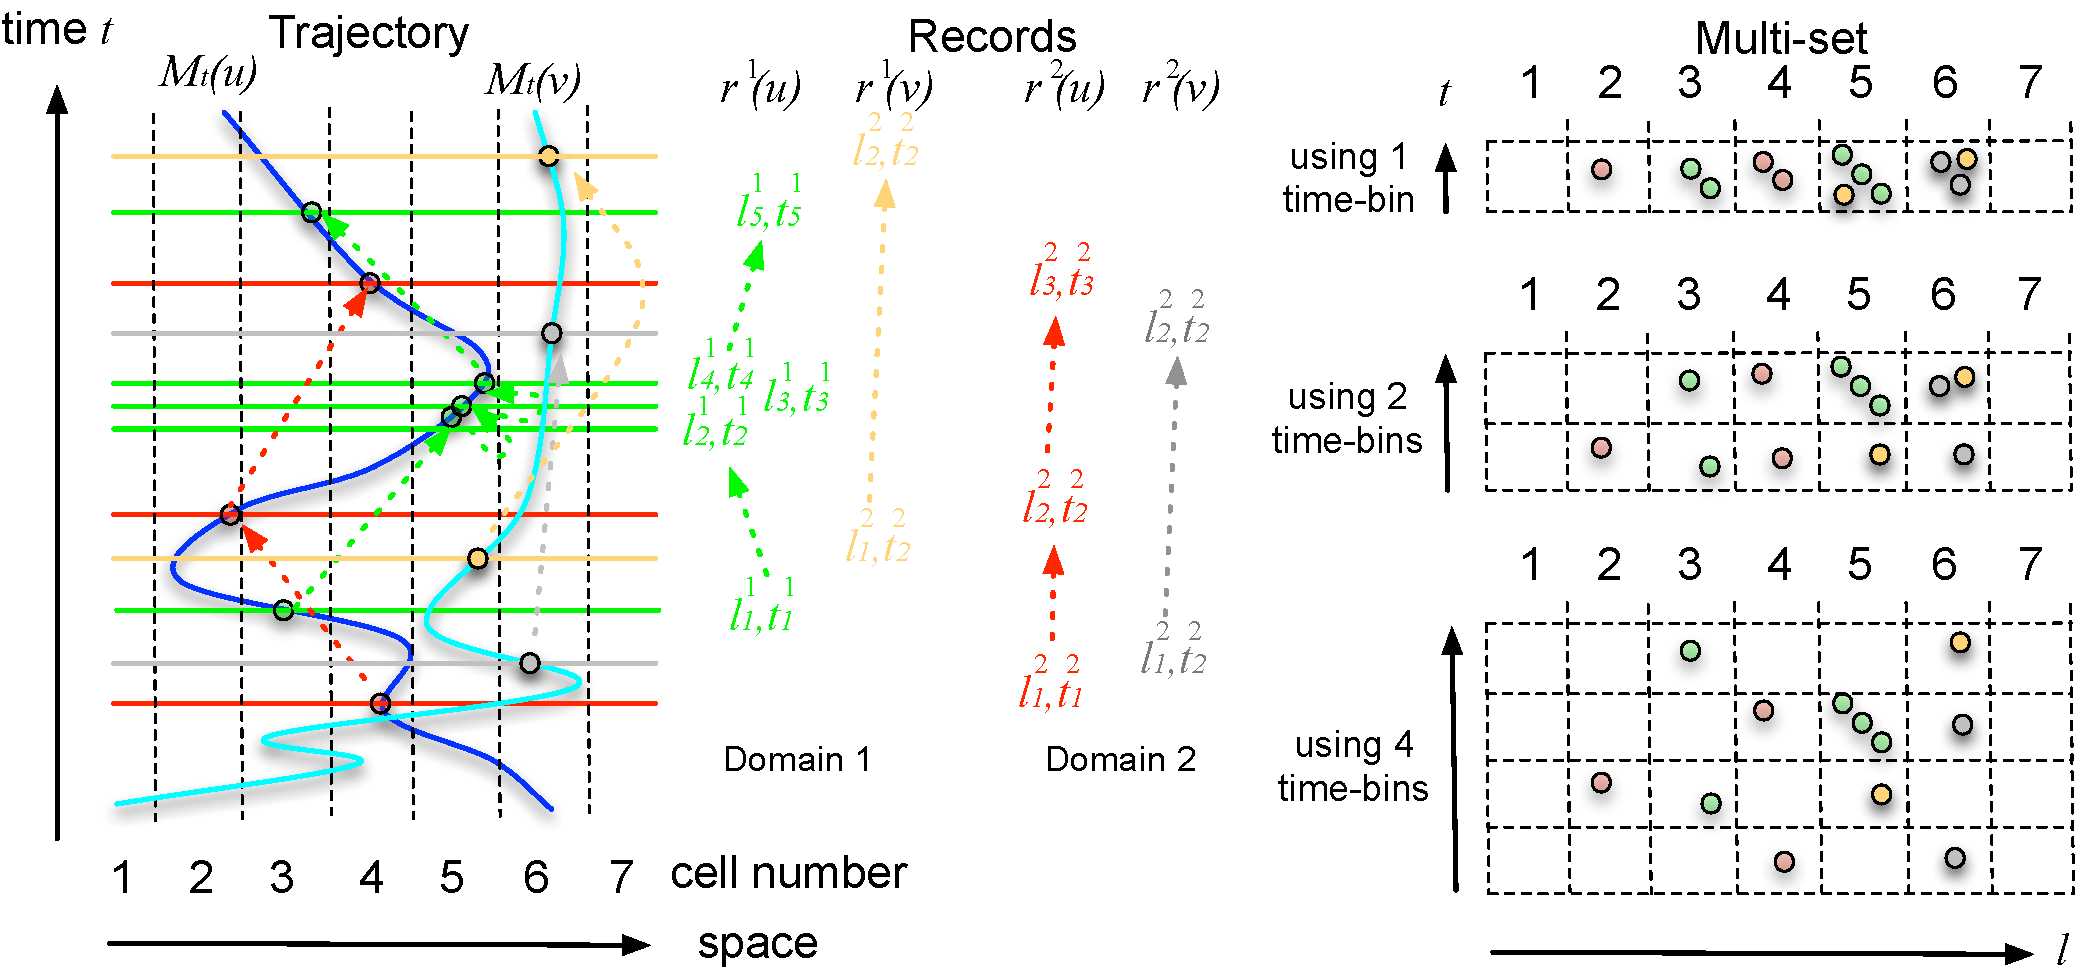
\includegraphics[width=0.65\linewidth]{fig/linking_explain.pdf}
  \end{center}
  \caption{Two space-time trajectories with associated footprints in two domains.}
  \label{fig:linking_explain}
\end{figure*}

% Describe problem
We formalized the problem in the following manner.
We defined $U$ and $V$ to be sets of $n$ user accounts in two separate domains.
Each account is a itself a set of spatiotemporal points $p$, where
\[ p = \langle u, l, t \rangle \]
with $u$ being a user ID unique to either $U$ or $V$, $l$ is a location, and $t$ is a time.
We denoted $\sigma_I$ to be a true (``identity'') mapping that correctly links the two accounts of the each user across $U$ and $V$.
The goal then, of this work, is to recover $\sigma_I$.
    
We made a series of simple assumptions about human mobility.
We broke time into discrete ``bins" of a certain length, and then declared the number of checkins a user has at each location in time bin to be Poisson distributed according to a rate paramater $\lambda$ unique to that time and place.
This is a simple but reasonable assumption, and Poisson distributions are often used to model rare events (like checkins).

This model generates the \emph{real world} mobility of a user.
We assume that this real world mobility is sampled independentally and randomly for the two different data sets with probability $p_U$ and $p_V$.

\fig{fig:linking_explain} provides a visual illustration.
On the left side of the image are two real world trajectories, denoted with a blue and turquoise line.
The x axis shows space and the y axis shows time.
The colored circles (red, green, gray and yellow) show times and places where the real world trajectories are sampled, with (for example) a geolocated photograph, phone call, or checkin.
The challenge is that we only see the green, yellow, red, and gray trajectories in the middle of the image, and we must figure out the true association across datasets.
In this example, red should go with green and gray with yellow.
On the right side of the image, the concept of time bins are illustrated.
We discretize time with varying sized time bins.
The top uses one large time bin, essentially ignoring time, whereas the bottom breaks time into four sections, essentially saying two locations are only the same if the checkins occur near one another in time.

% Describe algorithm
% Based on these assumptions, we were able to develop a maximum likelihood 

% Describe dataset
\begin{table*}
  \centering
  \begin{tabular}{llrrrrr}
    % \toprule
            &        & Number & Number  &   Median  &  Number   &           \\
    Dataset & Domain & Users & Checkins &  Checkins & Locations & Date Range\\
    \midrule
    FSQ-TWT   & Foursquare  & 862 & 13,177  & 8    & 11,265 & 2006-10 -- 2012-11 \\
              & Twitter     & 862 & 174,618 & 60.5 & 75,005 & 2008-10 -- 2012-11 \\
    \addlinespace
    IG-TWT    & Instagram   & 1717 & 337,934 & 93 & 177,430 & 2010-10 -- 2013-09 \\
              & Twitter     & 1717 & 447,366 & 89 & 182,409 & 2010-09 -- 2015-04 \\
    \addlinespace
    Call-Bank & Phone Calls       & 452 & $\sim$200k & $\sim$550 & $\sim$3500 & 2013-04 -- 2013-07 \\
              & Card Transactions & 452 & $\sim$40k & $\sim$60 & $\sim$3500 & 2013-04 -- 2013-07 \\
    % \bottomrule
  \end{tabular}
  \caption{Overview of datasets used in study. For FSQ-TWT and IG-TWT, number of locations refers to locations at a 4 decimal GPS granularity (position within roughly 10m).}
  \label{tab:link-data}
\end{table*}

We evaluated this algorithm on multiple real-world datasets.
Gathering the data in itself was a significant challenge, as each dataset needed to contain individuals with identities linked across two different data sources.
Collecting information from one data source is enough of a challenge by itself, given unexpected and changing data formats, connectivity problems, rate limits, and more.
Getting ground truth data across two datasets is thus more difficult, as two APIs need to be dealt with and user identities must be verified across the two.

We gathered three datasets:
\begin{itemize}
  % Data from foursquare checkins and geolocated tweets, from another paper.
  \item \textbf{Foursquare-Twitter} (FSQ-TWT): 
  checkin data from the location-based social networking and review site Foursquare \footnote{\url{https://foursquare.com/}} and geotagged updates from the microblogging site Twitter \footnote{\url{twitter.com}}. 
  This data was obtained in a prior work by other authors who allowed us to use their data~\cite{Zhang:2014ij}.
  We expect the behavior to be somewhat different across the two networks; Foursquare is primarily used to review restaurants, and Twitter is generally used.

  % Geolocated photos and geolocated tweets. Not the exact same. Got twitter account from profile. Medium difficulty.
  \item \textbf{Instagram-Twitter} (IG-TWT):
  Geolocated photographs from the image sharing site Instagram \footnote{\url{instagram.com}} and geotagged updates from the microblogging site Twitter.
  We first crawled Instagram, and then found users who had posted their Twitter usernames in their profiles.
  For each of these users, we used Twitter's API to crawl their public tweets.
  We expected this dataset to be the easiest to link, as there were high numbers of checkins on both sites for most users.

  % Cell phone calls (located to cell tower) and geocoded businesses.
  \item \textbf{Cell phone-Credit Card} (Call-Bank):
  Phone calls associated with geolocated cell towers (CDR) and credit or debit card transaction data associated with geocoded businesses, all from one G20 country.
  Locations were declared the same if the lat-lon of business was within a cell created via a Voronoi tesselation.
  This data was very sparse and the behaviors generating data seems to be very different in the two sets, making us hypothesize that we would have our worst results on it.
\end{itemize}

Statistics about these datasets is summarized in Table~\ref{tab:link-data}.

% Describe results
\begin{figure*}[th!]
  \centering
  \hspace{-0.7cm}
  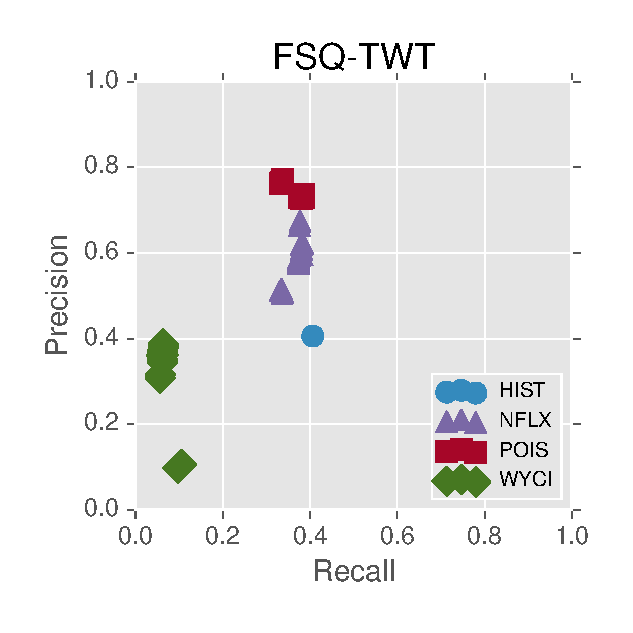
\includegraphics[width=0.35\linewidth]{fig/fs_scatter.eps}
  \hspace{-0.7cm}
  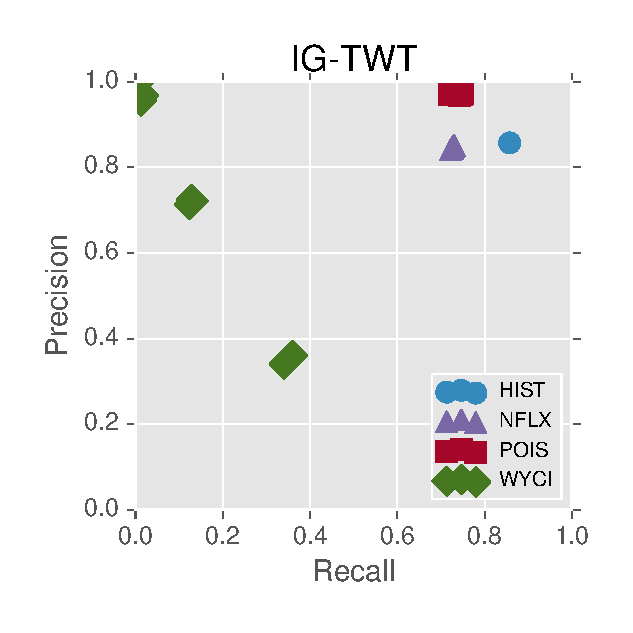
\includegraphics[width=0.35\linewidth]{fig/ig_scatter.eps}
  \hspace{-0.7cm}
  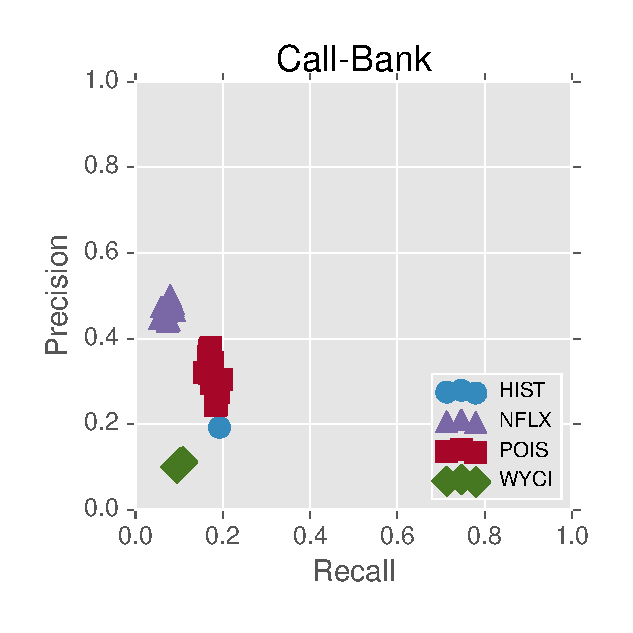
\includegraphics[width=0.35\linewidth]{fig/gd_scatter.eps}
  \caption{Precision and Recall plots for each dataset.}
  \vspace{1ex}
  \label{fig:link-prec-recall}
\end{figure*}

We now turn our attention to experimental performances of our algorithm. 
In Figure~\ref{fig:link-prec-recall}, we show the precision recall plots for our algorithm (for different eccentricity values) and for the other three reconciliation techniques: HIST, NFLX and WYCI. 
For our algorithm, we used estimated parameters and  for the other techniques, we used optimal parameters (found via exhaustive search).

There are several interesting observations that we can make on Figure~\ref{fig:link-prec-recall}. 
First, on the public dataset FQ-TWT our algorithm outperforms all prior methods (especially in precision). 
Nevertheless it is interesting to note that the precision of all methods is not ideal, probably due to sparsity of the data.

A second interesting observation is that our algorithm achieves very high precision when the dataset is more rich. 
In fact when we then turn our attention to our second dataset, the live service (IG-TWT) that we crawled, we obtain almost perfect precision. 
Note that not all the other techniques, for example NFLX, are able to leverage the denser data, as much.

Finally we test our method on a much more heterogeneous dataset (Call-Bank) that is also more realistic and sensitive. 
In this setting our algorithm outperforms previous techniques, with none of the previous algorithms able to achieve good precision and recall at the same time. 

% TODO(can possible add more results)
Additional results fully described in the paper found that our algorithms rapidly improved with more data.
Additionally, varying the size of timebins or the eccentricity parameter or number of terms did not have a large impact on results, meaning our algorithm's performance should remain stable to different sets of parameters.

